\chapter{Biltegiratze lokala, localStorage APIa}
\index{localStorage}\index{stateless}

HTTP protokoloak ez du memoriarik. Eskaera baten eta ondorengoen artean protokoloak ez du ezer gogoratzen, hau da, \textit{stateless} protokoloa dela esaten dugu. Adibide batekin aztertuko dugu hau. Demagun hiru web orri ditugula (ikus \ref{fig:localstorage1}. irudia):

\begin{figure}[ht]
	\centering
\begin{tikzpicture}
\node[anchor=south west,inner sep=0] (image) at (0,0)
   {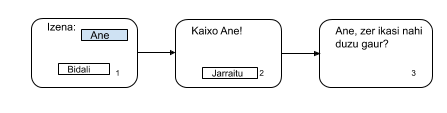
\includegraphics[trim=0cm 0cm 0cm 0cm, clip=true, width=.75\textwidth]{img/localstorage/localstorage1.png}};
\end{tikzpicture}
\caption{HTTP protokoloak ez du memoriarik. Formulario batek jasotzen duen informazioa bistaratzeko ez dago arazorik, baina 3. pantaila batera informazio hori bidaltzeko bai, ordea.}
\label{fig:localstorage1}
\end{figure}


Lehenengo orrian, erabiltzaileari izena eskatzen zaio. Kasu honetan ``Ane'' idatzi, \hl{Bidali} botoian sakatu eta bigarren orrira goaz. Bertan zerbitzariak ``Kaixo Ane!'' idatzi behar du eta jarraitzeko botoi bat eskaini. Hau lortzeko ez dugu arazorik, ``Ane'' izena parametro gisa baitoa formularioan. Baina bigarren orritik hirugarren orrirako jauzian, nola bidali ``Ane'' izena? Aukera bat izan daiteke \mbox{\textit{hidden}} motako eremu batean bidaltzea. Baina badago beste aukera bat sartu ditugun datuak HTTP zerbitzariari gogorarazteko: cookieak \index{cookie} erabiltzea. Honela funtzionatuko du (ikus \ref{fig:localstorage2} irudia):

\begin{figure}[ht]
	\centering
\begin{tikzpicture}
\node[anchor=south west,inner sep=0] (image) at (0,0)
   {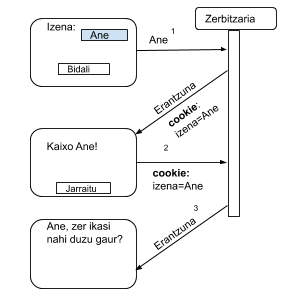
\includegraphics[trim=0cm 0cm 0cm 0cm, clip=true, width=.35\textwidth]{img/localstorage/localstorage2.png}};
\end{tikzpicture}
\caption{HTTP protokoloan egoera mantentzeko cookieak erabiltzen ohi dira.}
\label{fig:localstorage2}
\end{figure}


Erabiltzaileak Ane izena sartu eta Bidali botoian sakatu ondoren, zerbitzariak ``Ane'' parametroa jaso eta erabiltzaileari hurrengo orria bidaltzen dio, cookie batekin batera (cookiearen balioa izena=Ane delarik). Erabiltzailearen nabigatzaileak, hemendik aurrera, zerbitzari horri edozein gauza eskatzearekin batera beti bidaliko dio jaso duen cookiea, lekuko bat izango balitz bezala. Bigarren pausoan zerbitzariak cookiea jaso eta izena=Ane ikusita badaki zeinek bidali dion. Gauzak horrela, azken (hirugarren) orrialdea prestatu eta nabigatzaileari bidaliko dio, 
``Ane, zer ikasi nahi duzu gaur'' testuarekin batera. Landu dugun adibide honen inplementazioarekin praktikatzeko, hemengo\footnote{https://gist.github.com/juananpe/824b1d9ad2141d5c64bc8693492863f9} kodea erabili (martxan ikusi nahiko bazenu, Heroku aplikazio honetan \footnote{https://mighty-anchorage-92406.herokuapp.com/} argitaratu da).

Beraz, cookieek informazioa gordetzeko balio dute, eta, horrekin batera, HTTP protokoloari egoera gogoratzeko bide bat emango diogu. % Cookieek saioak gordetzeko ere balioko dute baina hori beste gai batean jorratuko da. 

\begin{alertinfo}{Informazio pribatua eta cookieak}
Adi! Ez gorde informazio pribatua cookie baten barruan (adibidez, ez gorde inoiz pasahitzak cookie baten barruan). Horren ordez, cookiean identifikatzaile bat gorde dezakegu eta zerbitzariaren lana izango da cookie horren identifikatzaileari edukia esleitzea eta gordetzea. Horrela, informazio pribatua zerbitzarian gordeko da beti, eta ez bezeroan. 
\end{alertinfo}

Cookie baten tamaina maximoa 4 KB da, beraz biltegiratze lokala lortzeko ez du askotarako ematen. Baina HTML5ek beste API bat eskaintzen du datuak bezeroan gorde eta kudeatu ahal izateko, Web Storage API \index{Web Storage API} delakoa.

\section{Web Storage APIa}

API honek \textit{izena=balioa} formatuari jarraitzen dioten balioen biltegiratze lokala (\textit{localStorage} \index{localStorage} delakoa) ahalbidetzen du. Domeinu bakoitzeko 5-10 MB gorde ditzake nabigatzailean bertan. Cookieekin ez bezala, behar direnean erabiltzen dira (gogoratu cookieen kasuan nabigatzaileak beti bidali behar zituela zerbitzarira).

\textit{LocalStorage} biltegian idazteko \textit{setItem} \index{setItem} metodoa erabiliko dugu:

\begin{lstlisting}[language=javascript,numbers=none]
localStorage.setItem("gakoa", balioa);
\end{lstlisting}

Eta balio bat irakurtzeko, \textit{getItem}:
\index{getItem}
\begin{lstlisting}[language=javascript,numbers=none]
let balioa = localStorage.getItem("gakoak");
\end{lstlisting}
 
LocalStorage array bat izango balitz bezala ere trata daiteke, bai datuak irakurtzeko:

\begin{lstlisting}[language=javascript,numbers=none]
let balioa  = localStorage["gakoa"];
\end{lstlisting}

nola gordetzeko:

\begin{lstlisting}[language=javascript,numbers=none]
localStorage["gakoa"] = balioa;
\end{lstlisting}

Balio bat localStorage-tik ezabatzeko, \textit{removeItem}  \index{removeItem} erabiliko dugu:

\begin{lstlisting}[language=javascript,numbers=none]
localStorage.removeItem("gakoa");
\end{lstlisting}


Posible da, halaber, localStorage biltegian dauden aldagai guztiak ezabatzea, \textit{clear} metodoarekin \index{clear}:

\begin{lstlisting}[language=javascript,numbers=none]
localStorage.clear();
\end{lstlisting}

\textit{length} atributua eta \textit{key()} metodoaren laguntzaz, localStorage biltegiko balioak zeharka ditzakegu \index{length}\index{key}:

\begin{lstlisting}[language=javascript,numbers=none]
for (let i=localStorage.length; i >= 0; i--){
    let gakoa = localStorage.key(i);
    console.log( localStorage.get(gakoa) );
}
\end{lstlisting}

\subsection{Nola aztertu localStorage biltegian dagoen edukia}

Firefox-en \textit{Biltegiratzea} izeneko erlaitzean, \textit{Biltegiratze lokala} atalean aurkituko dugu localStorage biltegia, domeinuka antolatuta. Adibidez, \ref{fig:localstorage3} irudian, berria.eus webgunean sartzean gordetzen den informazioa ikus daiteke.

\begin{figure}[ht]
	\centering
\begin{tikzpicture}
\node[anchor=south west,inner sep=0] (image) at (0,0)
   {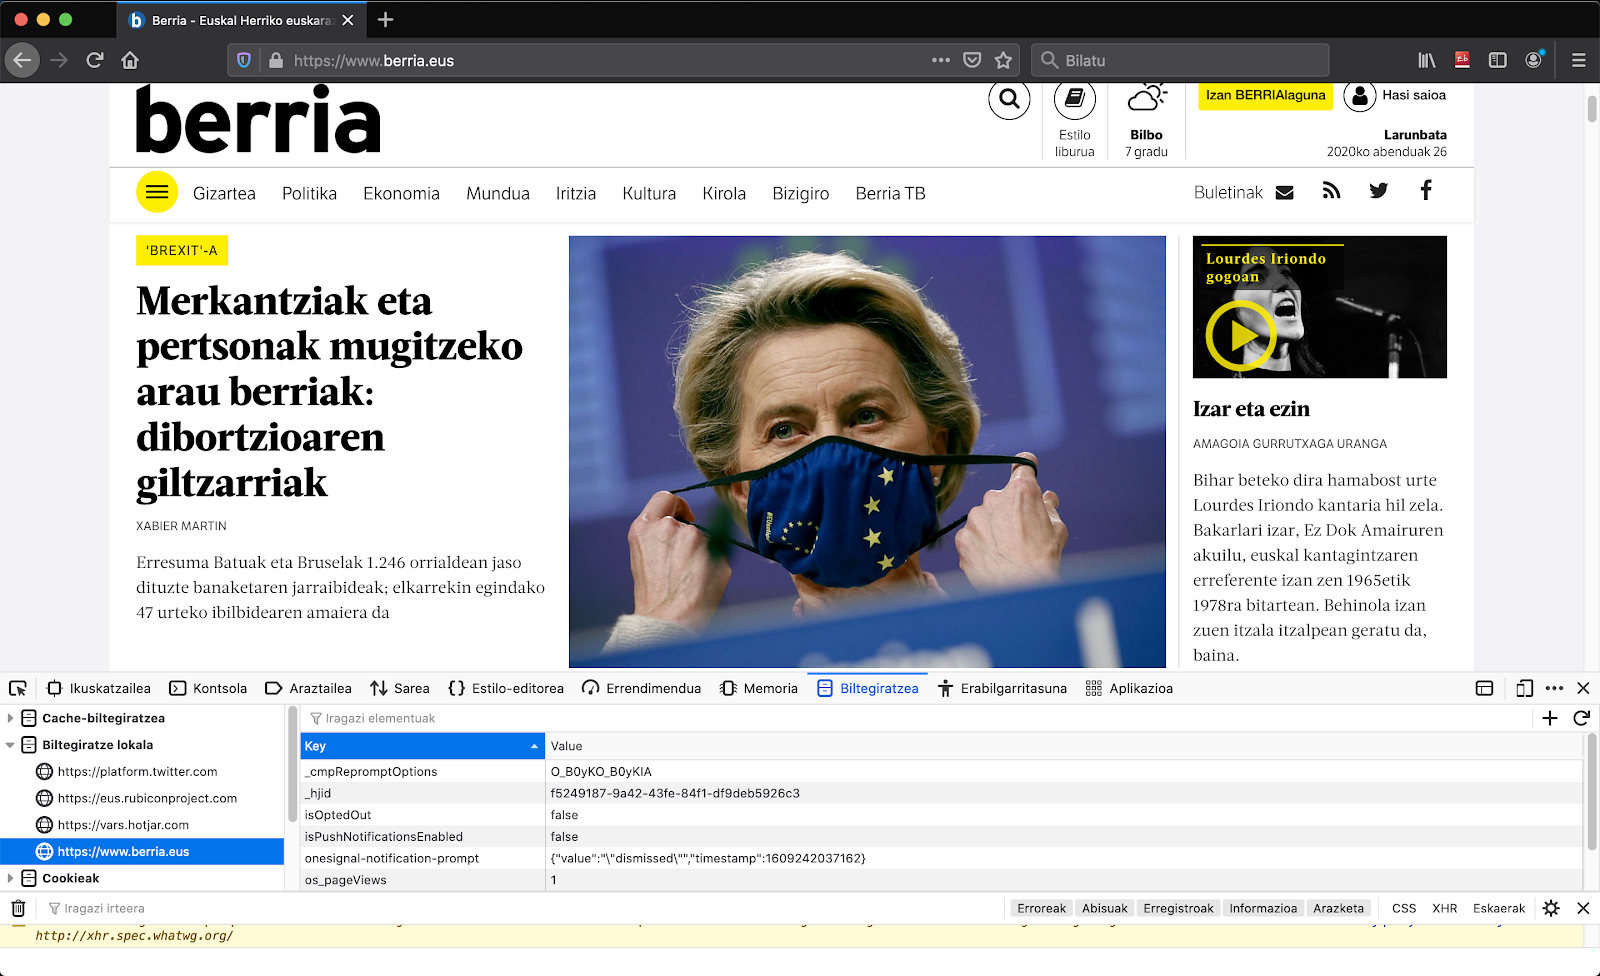
\includegraphics[trim=0cm 0cm 0cm 0cm, clip=true, width=.70\textwidth]{img/localstorage/localstorage3.png}};
\end{tikzpicture}
\caption{Berriak localStorage erabiltzen du hainbat informazio nabigatzailean bertan gordetzeko, besteak beste erabiltzailearen baimena (\textit{push})\index{push} jakinarazpenak jaso nahi dituen edo ez zehazteko.}
\label{fig:localstorage3}
\end{figure}

Kontsolan \textit{localStorage.clear()} \index{clear} metodoari deitzean, bertan zeuden datu guztiak ezabatu ahalko ditugu.

% \begin{figure}[ht]
% 	\centering
% \begin{tikzpicture}
% \node[anchor=south west,inner sep=0] (image) at (0,0)
%    {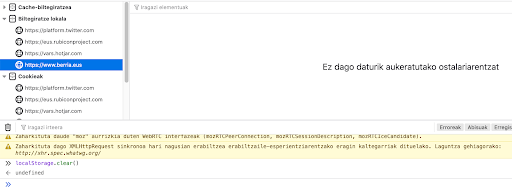
\includegraphics[trim=0cm 0cm 0cm 0cm, clip=true, width=.5\textwidth]{img/localstorage/localstorage4.png}};
% \end{tikzpicture}
% \caption{localstorage4}
% \label{fig:localstorage4}
% \end{figure}

LocalStorage biltegia hutsik dagoelarik, berriro kargatzen badugu berria.eus webgunea, Berriak (push) jakinarazpenak jaso nahi ditugun galdetuko digu (\ref{fig:localstorage5} irudia). 


\begin{figure}[ht]
	\centering
\begin{tikzpicture}
\node[anchor=south west,inner sep=0] (image) at (0,0)
   {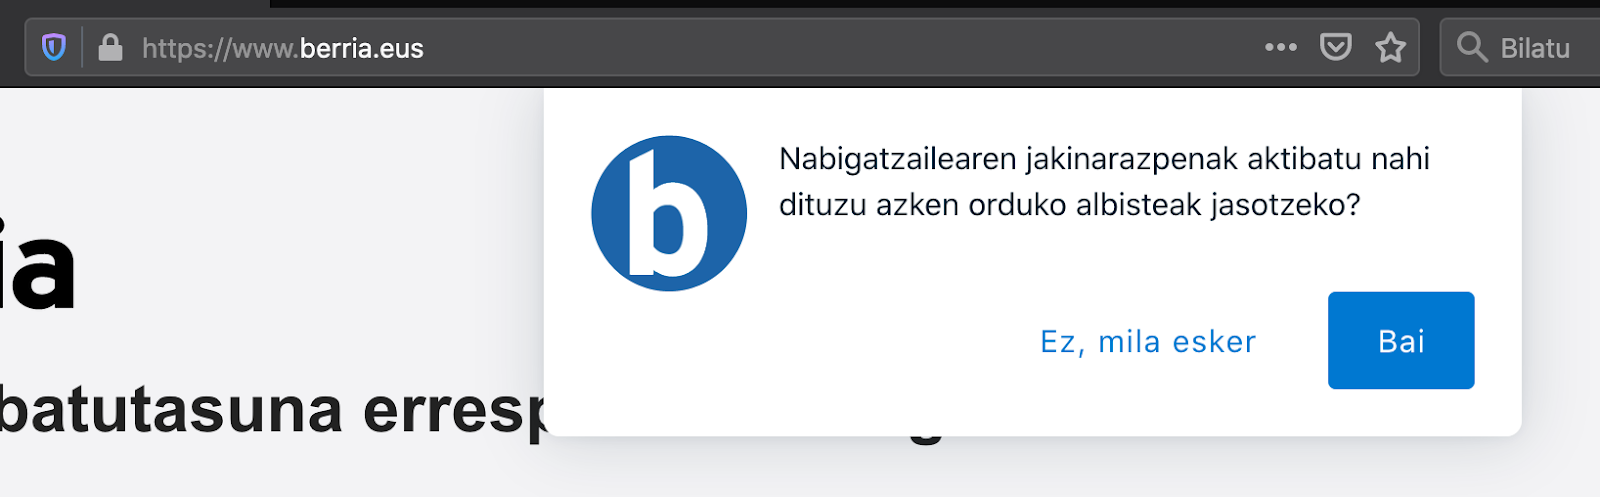
\includegraphics[trim=0cm 0cm 0cm 0cm, clip=true, width=.5\textwidth]{img/localstorage/localstorage5.png}};
\end{tikzpicture}
\caption{Berriak push jakinarazpenak jaso nahi ditugun edo ez galdetuko digu lehendabiziko bisitan. Erabiltzailearen erantzuna localStorage biltegian gordetzen da (horrela ez zaio berriro ere galdetuko hurrengo bisitan).}
\label{fig:localstorage5}
\end{figure}

% Dirudienez localStorage-n gordetzen du jakinarazpenak jaso nahi ditugun edo ez, isPushNotificationsEnabled aldagaian:
% 
% \begin{figure}[ht]
% 	\centering
% \begin{tikzpicture}
% \node[anchor=south west,inner sep=0] (image) at (0,0)
%    {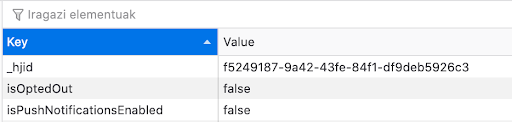
\includegraphics[trim=0cm 0cm 0cm 0cm, clip=true, width=.5\textwidth]{img/localstorage/localstorage6.png}};
% \end{tikzpicture}
% \caption{localstorage6}
% \label{fig:localstorage6}
% \end{figure}

\newpage
\section{Ariketak}

OpenLibrary APIa erabil dezakegu liburu baten datuak lortzeko bere ISBNa pasatuz. Adibidez:
 
 
\begin{lstlisting}[language=javascript,numbers=none]
 fetch("https://openlibrary.org/api/books? bibkeys=ISBN:9781491906187&
 jscmd=details&format=json").then( r=> r.json()).then( r => console.log (r['ISBN:9781491906187'].details))
\end{lstlisting}
   
    

% \begin{figure}[ht]
% 	\centering
% \begin{tikzpicture}
% \node[anchor=south west,inner sep=0] (image) at (0,0)
%    {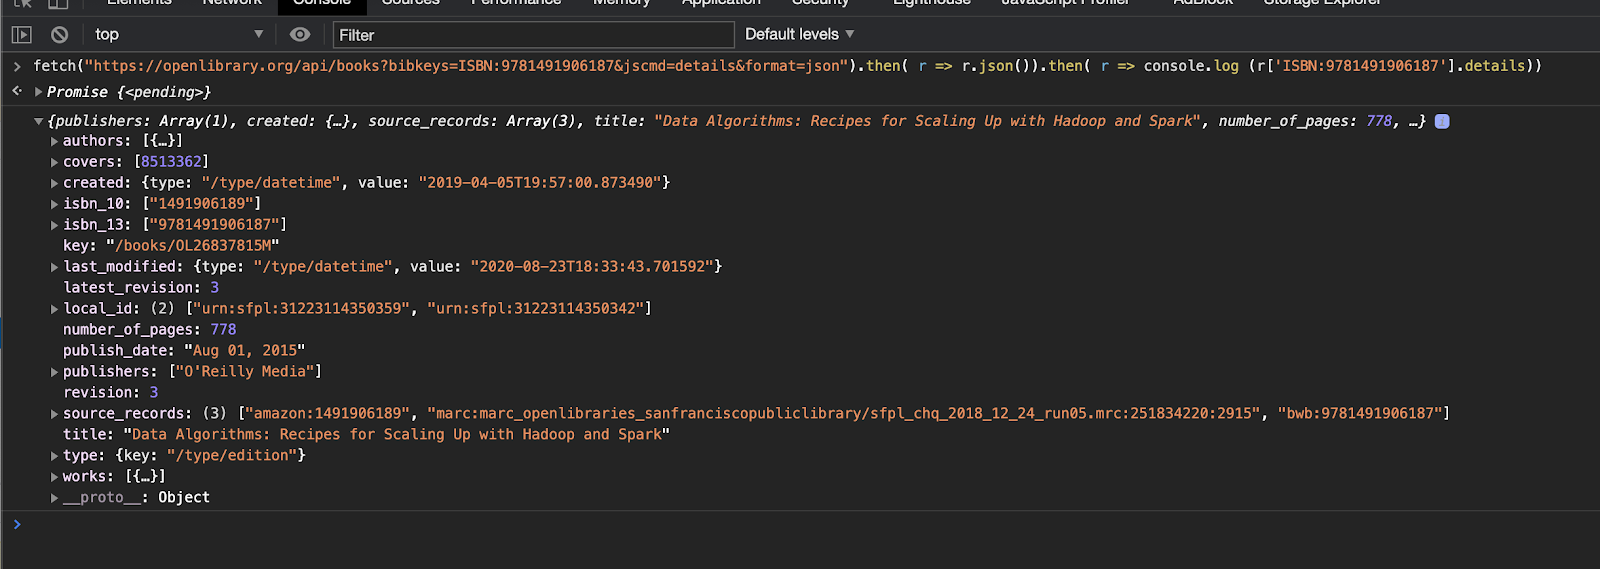
\includegraphics[trim=0cm 0cm 0cm 0cm, clip=true, width=.75\textwidth]{img/localstorage/localstorage7.png}};
% \end{tikzpicture}
% \caption{OpenLibrary APIa erabiliz liburu baten metadatuak jaso ditzakegu. Horiek localStorage biltegian gordetzea da ariketa honen helburua.}
% \label{fig:localstorage7}
% \end{figure}
%

 OpenLibrary APIa erabiliz, egin ezazu programa bat ISBN array honetan dauden liburu guztien datuak localStorage biltegian gordetzeko:
 
\begin{lstlisting}[language=javascript,numbers=none] 
 ['ISBN:9781491906187', 'ISBN:9781491920497', 'ISBN:1491910399',
     'ISBN:1491946008', 'ISBN:1491978236', 'ISBN:9781491906187']
 \end{lstlisting}
 
 Bukatzean, dena ondo egin badugu, kode hau exekutatzean:
 
 \begin{lstlisting}[language=javascript,numbers=none]
 let liburua = localStorage.getItem( 'ISBN:9781491906187');
  console.log( liburua.title ); 
 \end{lstlisting}
 
 
 Emaitza hau jaso beharko genuke:
 "Data Algorithms: Recipes for Scaling Up with Hadoop and Spark".
 
 \textbf{Soluzioa}:
 \href{https://github.com/juananpe/express/blob/master/public/js/module.mjs}{https://github.com/juananpe/express/blob/master/public/js/module.mjs}
 
 
